\documentclass[12pt, titlepage]{article}

\usepackage{graphicx} % Allows for images
\usepackage{wrapfig} % Allows for text wrapping around images
\usepackage{hyperref} % Allows for hyperlinks
\usepackage{siunitx} % Allows for SI units
\usepackage{amsmath} % Allows for math
\usepackage{enumerate} % Allows for custom enumerations
\usepackage{xcolor} % Allows for custom colors
\usepackage{tikz, tcolorbox} % Allows for custom boxes
\usepackage{microtype} % Allows for better text alignment
\usepackage{listings} % Allows for code listings
\usepackage{booktabs} % Allows for better tables
\usepackage{float} % Allows for better figure placement
\usepackage{geometry} % Allows for custom page geometry
\usepackage{fancyhdr} % Allows for custom headers and footers
\usepackage{caption} % Allows for custom captions
\usepackage{array} % Required package for specifying column width and line in the table
\usepackage{changepage} % Required for the adjustwidth environment to temporarily widen margins

\fancypagestyle{myarticlestyle}{
    \fancyhf{} % Clear header and footer
    \fancyhead[L]{\leftmark} % Section name on the left
    \fancyhead[R]{\thepage} % Page number on the right
}
\fancypagestyle{tocstyle}{
    \fancyhf{} % Clear header and footer
    \fancyhead[L]{CONTENTS} % Section name on the left
    \fancyhead[R]{\thepage} % Page number on the right
}

\pagestyle{myarticlestyle}
\setlength{\headheight}{15pt}

\begin{document}
\tableofcontents
\listoffigures
\listoftables
\thispagestyle{tocstyle}
\newpage
\section{Objectives}
\begin{enumerate}
    \item \textbf{Determination of Buckling Loads:}
    \begin{itemize}
        \item Investigate and quantify the buckling loads of slender pin-ended bars through experimental procedures.
        \item Analyze the relationship between applied loads and the resulting center deflections for each tested bar.
    \end{itemize}

    \item \textbf{Comparison of Theoretical and Experimental Critical Loads:}
    \begin{itemize}
        \item Assess and calculate the theoretical critical loads for the pin-ended bars using relevant analytical models.
        \item Perform experimental tests to determine the critical loads for each bar.
        \item Conduct a comprehensive comparison between the theoretical predictions and the experimentally obtained critical loads for all tested bars.
    \end{itemize}
\end{enumerate}

Through these objectives, the aim is to enhance our understanding of the
buckling behavior of slender pin-ended bars and to evaluate the accuracy of
theoretical predictions in relation to practical experimental outcomes.
\newpage
\section{Procedure}
\begin{enumerate}
    \item \textbf{Bar Insertion and Setup:}
    \begin{itemize}
        \item Insert one of the bars between the supports, ensuring that the ball bearing at the ends seats firmly.
        \item Orient the larger dimension of the cross-section parallel to the floor.
        \item Position the displacement transducer to measure the vertical deflection of the bar.
    \end{itemize}

    \item \textbf{Moment of Inertia Calculation and Critical Load Prediction:}
    \begin{itemize}
        \item Calculate the minimum moment of inertia for the inserted bar.
        \item Predict the critical load for the bar based on the calculated moment of inertia.
    \end{itemize}

    \item \textbf{Data Collection Using Dalite Datascan Configurator:}
    \begin{itemize}
        \item Open the Dalite Datascan Configurator at the DB2Bc.OVL file.
        \item Click on the "monitor every second" window.
        \item Verify that the initial reading for the electrical potentiometer is zero.
        \item Apply the load increments slowly.
        \item At each increment, record the central deflection.
        \item Continue to increase the load until the column buckles or the central deflection becomes large.
    \end{itemize}

    \item \textbf{Repeat for All Bars:}
    \begin{itemize}
        \item Repeat steps 2 to 4 for all four bars in the experimental setup.
    \end{itemize}
\end{enumerate}

This procedure outlines the steps to insert the bars, calculate relevant
parameters, and conduct the experimental testing using the Dalite Datascan
Configurator. It ensures systematic data collection for each bar in the study.
\newpage
\section{Results}
\subsection{Plot Calibration Charts}
The calibration charts for the load cell and the displacement transducer are
shown in the subsequent figures. The calibration charts are used to determine
the equation of the line of best fit for the data points. The equation is then
used to calculate the load for any pressure values that exceeded those for
which the corresponding load is provided.
\subsubsection{Bar 1: 508 mm}
The calibration chart for the load cell of Bar 1 with 508 mm length is shown
in figure \ref{fig:bar1calib} along with the equation of the line of best fit.
\begin{figure}[H]
    \centering
    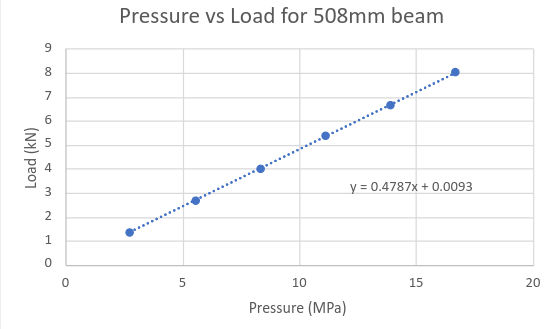
\includegraphics[width=0.8\textwidth]{./Images/508.png}
    \caption{Bar 1 Calibration Chart}
    \label{fig:bar1calib}
\end{figure}
\subsubsection{Bar 2: 737 mm}
The calibration chart for the load cell of Bar 2 with 737 mm length is shown
in figure \ref{fig:bar2calib} along with the equation of the line of best fit.
\begin{figure}[H]
    \centering
    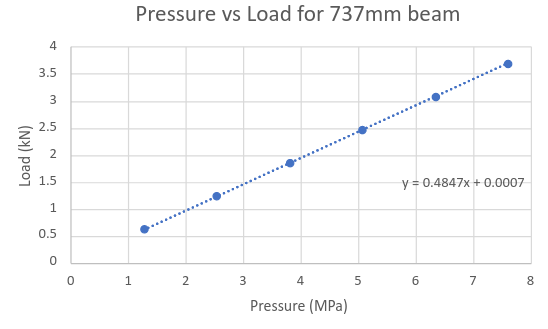
\includegraphics[width=0.8\textwidth]{./Images/737.png}
    \caption{Bar 2 Calibration Chart}
    \label{fig:bar2calib}
\end{figure}
\subsubsection{Bar 3: 902 mm}
The calibration chart for the load cell of Bar 3 with 902 mm length is shown
in figure \ref{fig:bar3calib} along with the equation of the line of best fit.
\begin{figure}[H]
    \centering
    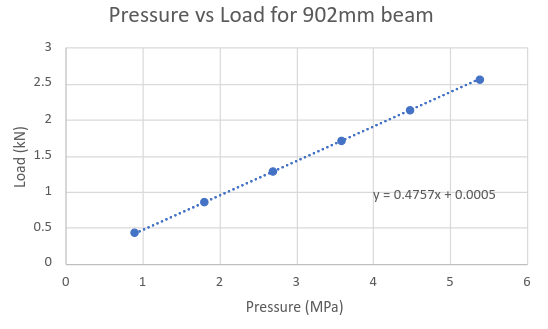
\includegraphics[width=0.8\textwidth]{./Images/902.png}
    \caption{Bar 3 Calibration Chart}
    \label{fig:bar3calib}
\end{figure}
\subsubsection{Bar 4: 997 mm}
The calibration chart for the load cell of Bar 4 with 997 mm length is shown
in figure \ref{fig:bar4calib} along with the equation of the line of best fit.
\begin{figure}[H]
    \centering
    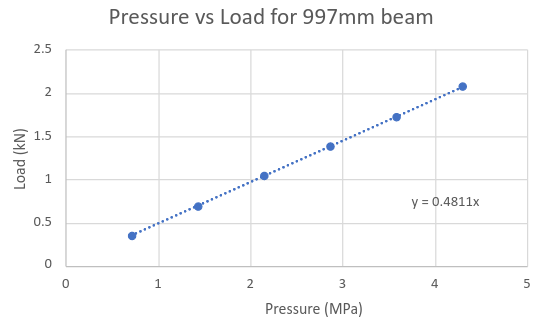
\includegraphics[width=0.8\textwidth]{./Images/997.png}
    \caption{Bar 4 Calibration Chart}
    \label{fig:bar4calib}
\end{figure}
\newpage
\subsection{Calculated Pressure for Exceeding Loads}
The pressure is calculated using the equation of the line of best fit for the
calibration charts. The calculated pressure is shown along with the load and
the deflection for each exceeding load in the subsequent tables.
\subsubsection{Bar 1: 508 mm}
The calculated pressure for the exceeding loads of Bar 1 with 508 mm length
is shown in table \ref{tab:bar1exceed}.
\begin{table}[H]
    \centering
    \caption{Bar 1: 508 mm Exceeding Loads}
    \label{tab:bar1exceed}
    \begin{tabular}{|c|c|c|}
        \hline
        \textbf{Pressure (MPa)} & \textbf{Load (kN)} & \textbf{Deflection (mm)}\\
        \hline
        2.785481949 & 1.34 & 0.3277 \\
        \hline
        5.570963899 & 2.68 & 0.7734 \\
        \hline
        8.356445848 & 4.015 & 1.271 \\
        \hline
        11.1419278 & 5.35 & 1.9436 \\
        \hline
        13.92740975 & 6.64 & 2.7734 \\
        \hline
        16.7128917 & 8.03 & 4.7394 \\
        \hline
        17.71952626 & 8.491637222 & 12.083 \\
        \hline
    \end{tabular}
\end{table}
\subsubsection{Bar 2: 737 mm}
The calculated pressure for the exceeding loads of Bar 2 with 737 mm length
is shown in table \ref{tab:bar2exceed}.
\begin{table}[H]
    \centering
    \caption{Bar 2: 737 mm Exceeding Loads}
    \label{tab:bar2exceed}
    \begin{tabular}{|c|c|c|}
        \hline
        \textbf{Pressure (MPa)} & \textbf{Load (kN)} & \textbf{Deflection (mm)}\\
        \hline
        1.268635343 & 0.616 & 0.2422 \\
        \hline
        2.537270687 & 1.23 & 0.6727 \\
        \hline
        3.80590603 & 1.845 & 1.2167 \\
        \hline
        5.074541373 & 2.46 & 1.6104 \\
        \hline
        6.343176716 & 3.075 & 2.1479 \\
        \hline
        7.61181206 & 3.69 & 2.7867 \\
        \hline
        10.06634566 & 4.879857741 & 23.3818 \\
        \hline
    \end{tabular}
\end{table}
\subsubsection{Bar 3: 902 mm}
The calculated pressure for the exceeding loads of Bar 3 with 902 mm length
is shown in table \ref{tab:bar3exceed}.
\begin{table}[H]
    \centering
    \caption{Bar 3: 737 mm Exceeding Loads}
    \label{tab:bar3exceed}
    \begin{tabular}{|c|c|c|}
        \hline
        \textbf{Pressure (MPa)} & \textbf{Load (kN)} & \textbf{Deflection (mm)}\\
        \hline
        0.896318449 & 0.427 & 0.1628 \\
        \hline
        1.792636898 & 0.853 & 0.2696 \\
        \hline
        2.688955347 & 1.28 & 0.4546 \\
        \hline
        3.585273796 & 1.707 & 0.6953 \\
        \hline
        4.481592245 & 2.13 & 1.2315 \\
        \hline
        5.377910694 & 2.56 & 5.1589 \\
        \hline
        7.322232253 & 3.483685883 & 18.8641 \\
        \hline
    \end{tabular}
\end{table}
\subsubsection{Bar 4: 997 mm}
The calculated pressure for the exceeding loads of Bar 4 with 997 mm length
is shown in table \ref{tab:bar4exceed}.
\begin{table}[H]
    \centering
    \caption{Bar 4: 997 mm Exceeding Loads}
    \label{tab:bar4exceed}
    \begin{tabular}{|c|c|c|}
        \hline
        \textbf{Pressure (MPa)} & \textbf{Load (kN)} & \textbf{Deflection (mm)}\\
        \hline
        0.717054759 & 0.345 & 0.1956 \\
        \hline
        1.434109519 & 0.69 & 0.6738 \\
        \hline
        2.151164278 & 1.035 & 1.0114 \\
        \hline
        2.868219037 & 1.38 & 1.3878 \\
        \hline
        3.585273796 & 1.725 & 1.9515 \\
        \hline
        4.302328556 & 2.07 & 2.4975 \\
        \hline
        6.343176716 & 3.051702318 & 20.7397 \\
        \hline
    \end{tabular}
\end{table}
\subsection{Analytical Calculations for Bar 1: 508 mm}
The following information is given:
\begin{itemize}
    \item $A = 12.7 \mathrm{mm} \times 19.07$ mm = 242.489 mm$^2$
    \item $E = 70$ GPa
    \item $L = 508$ mm
\end{itemize}
\subsubsection{Minimum Moment of Inertia}
The minimum moment of inertia is calculated using equation \ref{eq:mininertia}.
\begin{equation}
    \label{eq:mininertia}
    I_{min} = \frac{bh^3}{12}
\end{equation}
Substituting the values in equation \ref{eq:mininertia} yields equation
\ref{eq:bar1mininertia}.
\begin{equation}
    \label{eq:bar1mininertia}
    I_{min} = \frac{19.07 \times 12.7^3}{12} = 3255.2219 \mathrm{mm}^4
\end{equation}
\subsubsection{Critical Load}
The critical load is calculated using equation \ref{eq:critload}.
\begin{equation}
    \label{eq:critload}
    P_{cr} = \frac{\pi^2 EI_{min}}{L^2}
\end{equation}
Substituting the values in equation \ref{eq:critload} yields equation
\ref{eq:bar1critload}.
\begin{equation}
    \label{eq:bar1critload}
    P_{cr} = \frac{\pi^2 \times 70 \times 10^9 \times 3255.2219 \times 10^{-12}}{(508 \times 10^{-3})^2} = 8.7146 \mathrm{kN}
\end{equation}
\subsubsection{Critical Stress}
The critical stress is calculated using equation \ref{eq:critstress}.
\begin{equation}
    \label{eq:critstress}
    \sigma_{cr} = \frac{P_{cr}}{A}
\end{equation}
Substituting the values in equation \ref{eq:critstress} yields equation
\ref{eq:bar1critstress}.
\begin{equation}
    \label{eq:bar1critstress}
    \sigma_{cr} = \frac{8.71467 \times 10^3}{242.489} = 35.9829 \mathrm{MPa}
\end{equation}
\subsubsection{Radius of Gyration}
The radius of gyration is calculated using equation \ref{eq:radiusgyration}.
\begin{equation}
    \label{eq:radiusgyration}
    r = \sqrt{\frac{I}{A}}
\end{equation}
Substituting the values in equation \ref{eq:radiusgyration} yields equation
\ref{eq:bar1radiusgyration}.
\begin{equation}
    \label{eq:bar1radiusgyration}
    r = \sqrt{\frac{3255.2219}{242.489}} = 3.66617 \mathrm{mm}
\end{equation}
\subsubsection{Slenderness Ratio}
The slenderness ratio is calculated using equation \ref{eq:slenderness}.
\begin{equation}
    \label{eq:slenderness}
    \frac{L}{r} = \frac{508}{3.66617} = 138.564
\end{equation}
\subsection{Plot Load-Deflection Curves}
This section shows the load-deflection curves for each bar with an indication
of the critical load. Then, the percentage error between the theoretical and
experimental critical loads is calculated.
\subsubsection{Bar 1: 508 mm}
The load-deflection curve for Bar 1 with 508 mm length is shown in figure
\ref{fig:bar1loaddefl}. The theoretical critical load is 8.4916 kN and the
experimental critical load is 8.03 kN.
\begin{figure}[H]
    \centering
    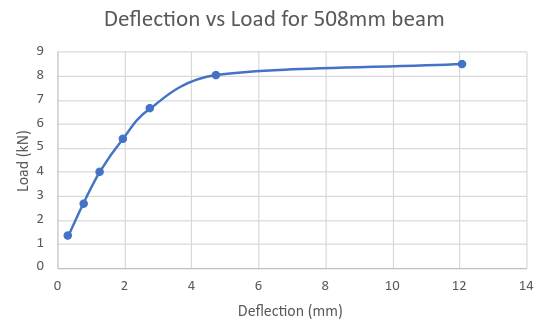
\includegraphics[width=0.8\textwidth]{./Images/d508.png}
    \caption{Bar 1: 508 mm Load-Deflection Curve}
    \label{fig:bar1loaddefl}
\end{figure}
The percentage error between the theoretical and experimental critical loads
is calculated using equation \ref{eq:percenterror} and is shown in equation
\ref{eq:bar1percenterror}.
\begin{equation}
    \label{eq:percenterror}
    \text{Percentage Error} = \frac{\text{Experimental} - \text{Theoretical}}{\text{Theoretical}} \times 100
\end{equation}
Substituting the values in equation \ref{eq:percenterror} yields equation
\ref{eq:bar1percenterror}.
\begin{equation}
    \label{eq:bar1percenterror}
    \text{Percentage Error} = \frac{\left| 8.03 - 8.4916\right|}{\left|8.4916\right|} \times 100 = 5.43\%
\end{equation}
\subsubsection{Bar 2: 737 mm}
The load-deflection curve for Bar 2 with 737 mm length is shown in figure
\ref{fig:bar2loaddefl}. The theoretical critical load is 4.8799 kN and the
experimental critical load is 3.69 kN.
\begin{figure}[H]
    \centering
    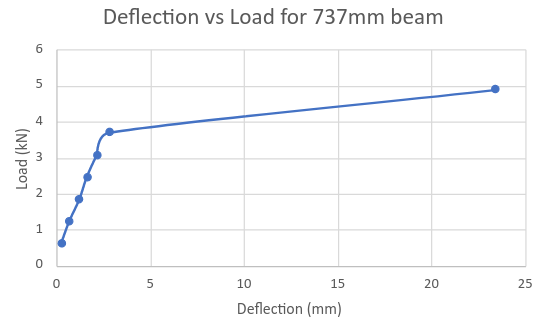
\includegraphics[width=0.8\textwidth]{./Images/d737.png}
    \caption{Bar 2: 737 mm Load-Deflection Curve}
    \label{fig:bar2loaddefl}
\end{figure}
The percentage error between the theoretical and experimental critical loads
is calculated using equation \ref{eq:percenterror} and is shown in equation
\ref{eq:bar2percenterror}.
\begin{equation}
    \label{eq:bar2percenterror}
    \text{Percentage Error} = \frac{\left| 3.69 - 4.8799\right|}{\left|4.8799\right|} \times 100 = 24.38\%
\end{equation}
\subsubsection{Bar 3: 902 mm}
The load-deflection curve for Bar 3 with 902 mm length is shown in figure
\ref{fig:bar3loaddefl}. The theoretical critical load is 3.4837 kN and the
experimental critical load is 2.56 kN.
\begin{figure}[H]
    \centering
    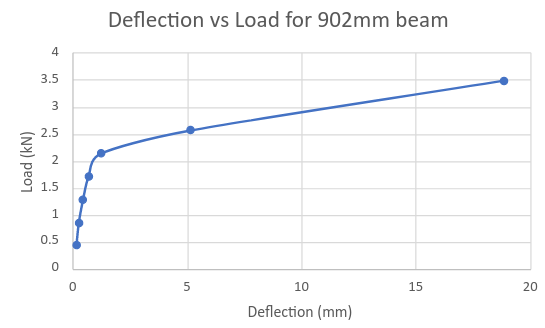
\includegraphics[width=0.8\textwidth]{./Images/d902.png}
    \caption{Bar 3: 902 mm Load-Deflection Curve}
    \label{fig:bar3loaddefl}
\end{figure}
The percentage error between the theoretical and experimental critical loads
is calculated using equation \ref{eq:percenterror} and is shown in equation
\ref{eq:bar3percenterror}.
\begin{equation}
    \label{eq:bar3percenterror}
    \text{Percentage Error} = \frac{\left| 2.56 - 3.4837\right|}{\left|3.4837\right|} \times 100 = 26.51\%
\end{equation}
\newpage
\subsubsection{Bar 4: 997 mm}
The load-deflection curve for Bar 4 with 997 mm length is shown in figure
\ref{fig:bar4loaddefl}. The theoretical critical load is 3.0517 kN and the
experimental critical load is 2.07 kN.
\begin{figure}[H]
    \centering
    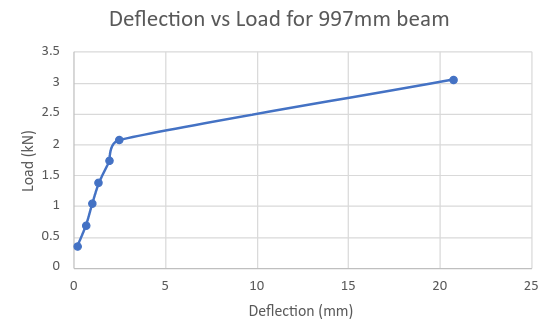
\includegraphics[width=0.8\textwidth]{./Images/d997.png}
    \caption{Bar 4: 997 mm Load-Deflection Curve}
    \label{fig:bar4loaddefl}
\end{figure}
The percentage error between the theoretical and experimental critical loads
is calculated using equation \ref{eq:percenterror} and is shown in equation
\ref{eq:bar4percenterror}.
\begin{equation}
    \label{eq:bar4percenterror}
    \text{Percentage Error} = \frac{\left| 2.07 - 3.0517\right|}{\left|3.0517\right|} \times 100 = 32.13\%
\end{equation}
\newpage
\subsection{Plot Critical Stress-Slenderness Ratio Curves}
This section shows the critical stress-slenderness ratio curves for each bar
for both the theoretical and experimental values in a single plot. The plot
is shown in figure \ref{fig:stressslenderness}.
\begin{figure}[H]
    \centering
    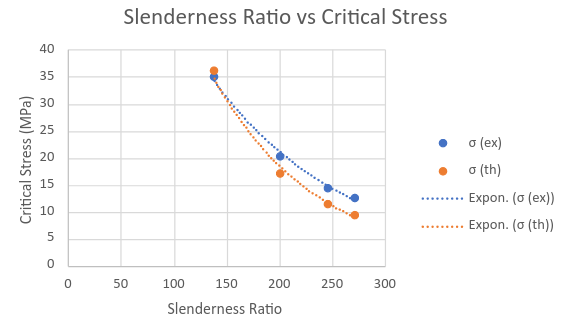
\includegraphics[width=0.8\textwidth]{./Images/s4.png}
    \caption{Critical Stress-Slenderness Ratio Curves}
    \label{fig:stressslenderness}
\end{figure}
\subsection{Summary of Results}
In this section, the pertinent results of the experiment are summarized in
a table. The table includes ($L$, $\frac{L}{r}$, $P_{cr,theo}$, $P_{cr,exp}$,
$\sigma_{cr,theo}$, $\sigma_{cr,exp}$, and \% Error). The summary table is
shown in table \ref{tab:summary}.
\begin{table}[H]
    \centering
    \caption{Summary of Results}
    \label{tab:summary}
    \begin{adjustwidth}{-1in}{-1in}
        \begin{tabular}{|c|c|c|c|c|c|c|c|}
            \hline
            \textbf{Bar} & \textbf{L (mm)} & \textbf{$\frac{L}{r}$} & \textbf{$P_{cr,theo}$ (kN)} & \textbf{$P_{cr,exp}$ (kN)} & \textbf{$\sigma_{cr,theo}$ (MPa)} & \textbf{$\sigma_{cr,exp}$ (MPa)} & \textbf{\% Error}\\
            \hline
            1 & 0.508 & 138.5640646 & 8.491637222 & 8.714670491 & 35.06202685 & 35.98293271 & 2.559285163 \\
            \hline
            2 & 0.737 & 201.0269992 & 4.879857741 & 4.140410674 & 20.14896523 & 17.09578335 & 17.85926868 \\
            \hline
            3 & 0.902 & 246.0330438 & 3.483685883 & 2.764173634 & 14.3841623 & 11.41329141 & 26.02992228 \\
            \hline
            4 & 0.997 & 271.945615 & 3.051702318 & 2.262497347 & 12.60049927 & 9.341866671 & 34.88202858 \\
            \hline
        \end{tabular}
    \end{adjustwidth}
\end{table}
\newpage
\section{Discussion}
\subsection{Results Discussion}
The experimental results indicate that the critical load decreases as the
length of the bar increases. This is consistent with theoretical predictions
and can be attributed to the increase in the slenderness ratio as the length
increases. The critical stress also decreases as the length increases, which
is also consistent with theoretical predictions. The percentage error between
the theoretical and experimental critical loads increases as the length
increases. This is likely due to the increased sensitivity of the longer bars
to environmental conditions and other factors that can affect the buckling
behavior.
\subsection{Sources of Error}
The percentage errors indicate variations between theoretical predictions and
experimental results. Factors such as:
\begin{itemize}
    \item \textbf{Environmental Conditions:} Variations in temperature, humidity, or other environmental factors can impact material behavior and measurements.

    \item \textbf{Alignment Issues:} Misalignment of experimental setup components, such as the load application system or displacement transducer, can lead to inaccuracies.

    \item \textbf{Instrumentation Limitations:} The precision and accuracy of measuring instruments, such as the load cell or displacement transducer, can introduce errors.

    \item \textbf{Boundary Conditions:} Deviations from idealized boundary conditions, such as perfectly pinned ends, can affect the buckling behavior.

    \item \textbf{Friction Effects:} Friction at the support points or between components can influence the buckling behavior.
\end{itemize}
Add to the errors between the theoretical and experimental results.\\[10pt]
Despite discrepancies, the experiment successfully demonstrated the buckling behavior
of slender pin-ended bars and provided insights into the accuracy of
theoretical predictions. Future work could focus on refining experimental
procedures and addressing sources of error for improved accuracy in
theoretical-experimental comparisons.
\newpage
\section{Conclusions}
The objectives of the experiment were successfully achieved. The buckling
behavior of slender pin-ended bars was investigated and quantified through
experimental procedures. The relationship between applied loads and the
resulting center deflections for each tested bar was analyzed. The theoretical
critical loads for the pin-ended bars were assessed and calculated using
relevant analytical models. Experimental tests were performed to determine
the critical loads for each bar. A comprehensive comparison between the
theoretical predictions and the experimentally obtained critical loads for
all tested bars was conducted. The experiment enhanced our understanding of
the buckling behavior of slender pin-ended bars and evaluated the accuracy
of theoretical predictions in relation to practical experimental outcomes.
\end{document}
